\section{Формула и произведение Ли}
\textbf{Вопрос.} Собирает ли формула те же числа, которые уже лежат в произведении Ли?

Формула говорит: равновесный $\delta$ сдвигается на $2\pi\xi_x/(C\eta_0)$ на единицу горизонтального действия, и на $-\eta_1\sigma_\delta^2/\eta_0$ на единицу синхротронного. Нормальная форма этих имён не использует: она усредняет лабораторный $\delta$ по фазам генераторов.

\begin{center}
\begin{tabular}{lcc}
\toprule
сдвиг $\delta_{\mathrm{eq}}$ на единицу действия & формула & нормальная форма \\
\midrule
горизонтальное действие & $\vdxForm$~м$^{-1}$ & $\vdxNF$ \\
вертикальное действие & $\vdyForm$~м$^{-1}$ & $\vdyNF$ \\
синхротронное действие & $\vdsForm$~м$^{-1}$ & $\vdsNF$ \\
\bottomrule
\end{tabular}
\end{center}

Относительная разница по горизонтали $\vdxRel$, по синхротрону $\vdsRel$. Это не таблица «насколько теория верна в процентах к трекингу»: это две записи одного сдвига.

\begin{figure}[H]\centering
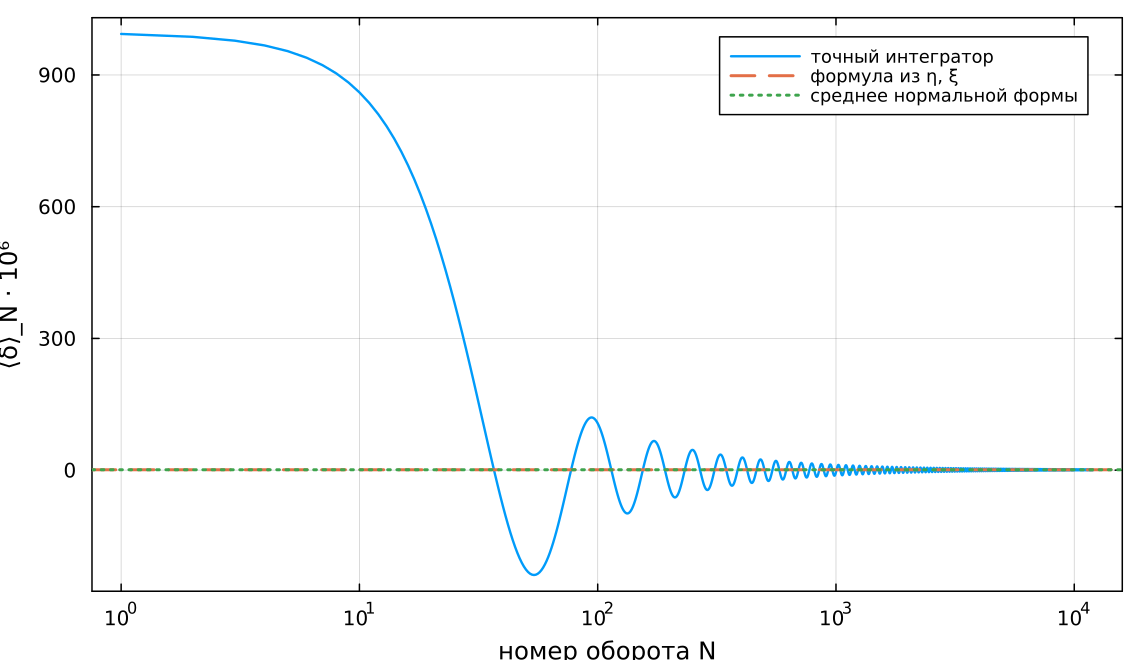
\includegraphics[width=0.92\textwidth]{figs/fig_07_lie.png}
\caption{Скользящее среднее интегратора и две горизонтали: формула из $\eta,\xi$ и среднее нормальной формы. Линия M2 посчитана из генераторов, без подстановки формулы.}
\end{figure}

\textbf{Вывод.} Формула собрала те же числа, которые алгебра уже содержит. Дальше среднее по оборотам садится на этот общий уровень.
